%%%%%%%%%%%%%%%%%%%%%%%%%%%%%%%%%%%%%%%%%%%%%%%%%%%%%%%%%%%%%%%%%%%%%%
% LaTeX Beamer Presentation based on Reservoir Computing Report
% Generated based on the provided main.tex report
%%%%%%%%%%%%%%%%%%%%%%%%%%%%%%%%%%%%%%%%%%%%%%%%%%%%%%%%%%%%%%%%%%%%%%

\documentclass{beamer}

% Theme selection (choose one, e.g., Madrid, Boadilla, Warsaw, etc.)
\usetheme{Madrid} % A popular theme with navigation bars [2]
\usecolortheme{rose} % A matching color theme [2]

% Packages from the report (add others if needed)
\usepackage{amsmath}
\usepackage{amsthm}
\usepackage{amsfonts}
\usepackage{amssymb}
\usepackage{graphicx} % For including images
\usepackage{booktabs} % For tables if needed
\usepackage{hyperref} % For links

% Math settings (optional, to make math fonts serif like in articles) [3]
% \usefonttheme{serif} % Uncomment if you prefer serif math fonts

% Report Information for Title Page
\title[Reservoir Computing]{Reservoir Computing: Implementation and Analysis}
\subtitle{Study Oriented Project - Presentation}
\author{Vimarsh Shah}
\institute{Department of Physics \\ BITS Pilani, Goa Campus}
\date{April 28, 2025}
\logo{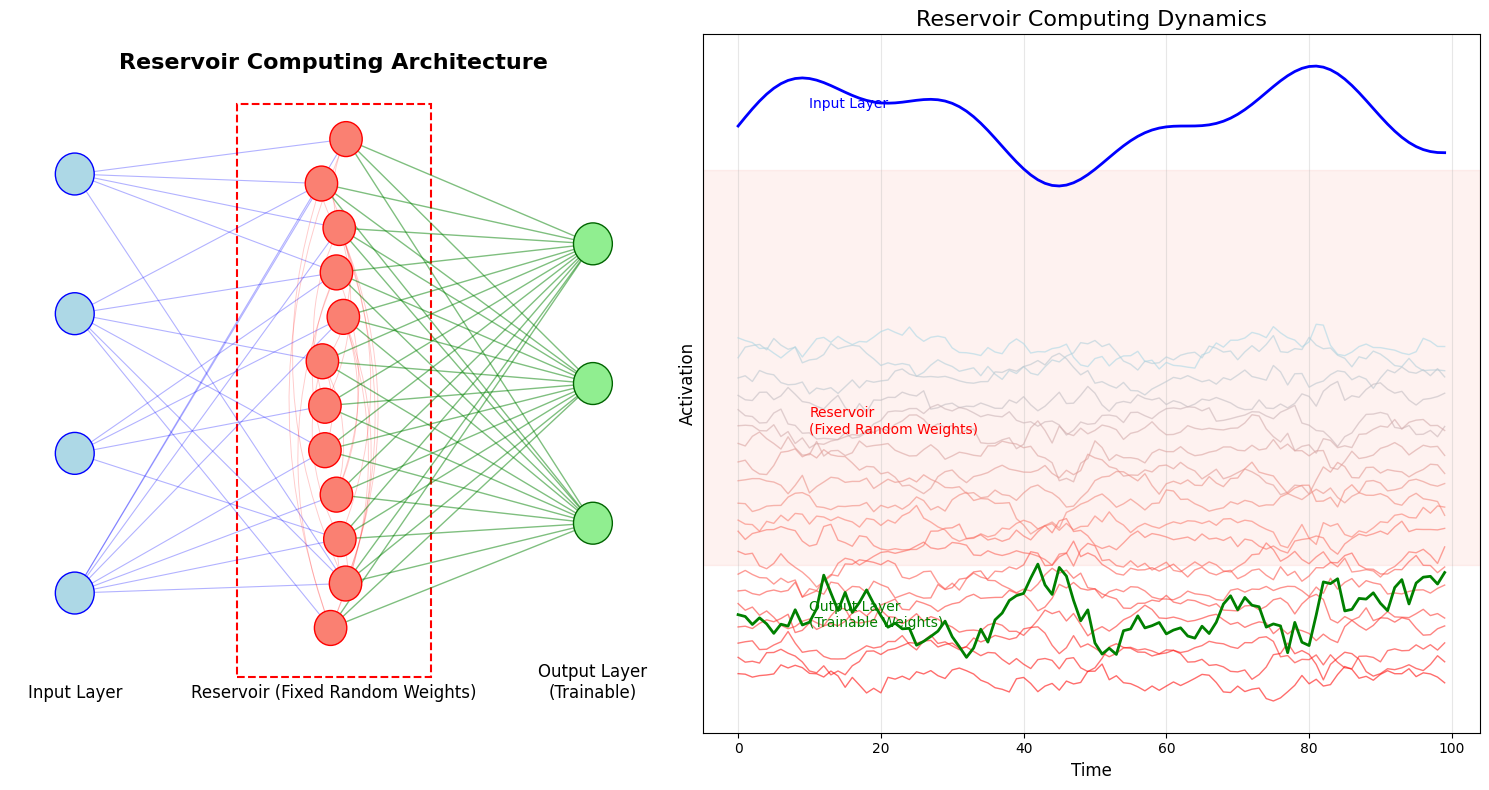
\includegraphics[height=1cm]{ivt-style/rc_intro_matplotlib}} % Use title figure as logo [2]

\begin{document}

% Title Page Frame
\frame{\titlepage} % [2]

% Table of Contents Frame
\begin{frame}
    \frametitle{Outline}
    \tableofcontents
\end{frame}

%%%%%%%%%%%%%%%%%%%%%%%%%%%%%%%%%%%%%%%%%%%%%%%%%%%%%%%%%%%%%%%%%%%%%%
% Section 1: Introduction
%%%%%%%%%%%%%%%%%%%%%%%%%%%%%%%%%%%%%%%%%%%%%%%%%%%%%%%%%%%%%%%%%%%%%%
\section{Introduction}

\begin{frame}
    \frametitle{Motivation: Machine Learning & Time Series}
    \begin{itemize}
        \item Machine learning excels at pattern extraction and prediction.
        \item Traditional Deep Learning often uses gradient-based optimization (backpropagation).
        \item Recurrent Neural Networks (RNNs) are designed for sequential/temporal data.
        \pause
        \item \textbf{Challenge:} Training RNNs is hard due to:
            \begin{itemize}
                \item Vanishing/exploding gradients.
                \item High computational cost.
            \end{itemize}
    \end{itemize}
\end{frame}

\begin{frame}
    \frametitle{Reservoir Computing (RC): An Alternative}
    \begin{itemize}
        \item RC maintains the power of recurrent networks but simplifies training.
        \item Key idea: Use a fixed, randomly initialized recurrent network (the \textbf{reservoir}).
        \item Only train the output connections (readout layer). \pause
        \item \textbf{Advantages:}
            \begin{itemize}
                \item Simplified training (often linear regression).
                \item Reduced computational cost.
                \item Inherent memory for temporal processing.
                \item Adaptable to physical hardware implementations.
            \end{itemize}
    \end{itemize}
\end{frame}

\begin{frame}
    \frametitle{Network Architectures Overview}
    \begin{figure}
        \centering
        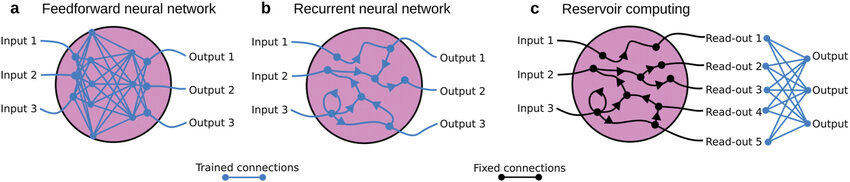
\includegraphics[width=1.0\linewidth]{figures/rc_difference_with others.png}
        \caption{Comparison: (a) Feedforward NN (FNN), (b) Recurrent NN (RNN), (c) Reservoir Computing (RC). Only RC readout (W\textsuperscript{out}) is trained.}
        \label{fig:rc_diff_slide}
    \end{figure}
\end{frame}

%%%%%%%%%%%%%%%%%%%%%%%%%%%%%%%%%%%%%%%%%%%%%%%%%%%%%%%%%%%%%%%%%%%%%%
% Section 2: Basics of Reservoir Computing
%%%%%%%%%%%%%%%%%%%%%%%%%%%%%%%%%%%%%%%%%%%%%%%%%%%%%%%%%%%%%%%%%%%%%%
\section{Basics of Reservoir Computing}

\begin{frame}
    \frametitle{General Principle}
    RC transforms inputs using a high-dimensional, nonlinear dynamical system (the reservoir).
    \begin{columns}[T] % Split frame into columns
        \begin{column}{0.4\textwidth} % Left column for text
            \textbf{Components:}
            \begin{itemize}
                \item \textbf{Input Layer:} Maps input $\mathbf{u}[n]$ to reservoir (fixed weights $\mathbf{W}^{\mathrm{in}}$).
                \item \textbf{Reservoir:} Recurrent network creates high-dimensional state $\mathbf{x}[n]$ (fixed weights $\mathbf{W}$).
                \item \textbf{Output Layer:} Linear readout maps reservoir state to output $\mathbf{y}[n]$ (trained weights $\mathbf{W}^{\mathrm{out}}$).
            \end{itemize}
        \end{column}
        \begin{column}{0.6\textwidth} % Right column for equations
            \textbf{Reservoir Update:}
            \[
            \mathbf{x}[n+1] = f\bigl(\mathbf{W}\mathbf{x}[n] + \mathbf{W}^{\mathrm{in}}\mathbf{u}[n] + \mathbf{b}\bigr)
            \]
            (\(f\) is e.g., $\tanh$)
            \pause\medskip
            \textbf{Output Calculation:}
            \[
            \mathbf{y}[n] = \mathbf{W}^{\mathrm{out}}\bigl[\mathbf{x}[n];\,\mathbf{u}[n]\bigr]
            \]
            (\(W^{\mathrm{out}}\) trained via linear regression)
        \end{column}
    \end{columns}
    \pause\bigskip
    \textbf{Key:} Internal dynamics ($\mathbf{W}, \mathbf{W}^{\mathrm{in}}$) are fixed and random, only $\mathbf{W}^{\mathrm{out}}$ is learned. Efficient!
\end{frame}

\begin{frame}
    \frametitle{Echo State Property (ESP) & Fading Memory}
    \begin{itemize}
        \item \textbf{ESP:} Ensures reservoir state depends on input history, not initial conditions.
            \begin{itemize}
                \item Influence of initial state fades away.
                \item Crucial for consistent processing of temporal data.
            \end{itemize}
        \pause
        \item \textbf{Fading Memory:} Reservoir retains information about recent inputs, with influence decaying over time.
            \begin{itemize}
                \item Essential for capturing temporal dependencies.
                \item Often achieved by ensuring spectral radius $\rho(\mathbf{W}) < 1$.
            \end{itemize}
        \pause
        \item \textbf{Balance Needed:} Sufficient memory capacity vs. nonlinearity for rich feature representation.
    \end{itemize}
\end{frame}

\begin{frame}
    \frametitle{Comparison with Traditional RNNs}
    \begin{tabular}{lp{5cm}p{5cm}}
        \toprule
        Feature & \textbf{Traditional RNNs} & \textbf{Reservoir Computing (RC)} \\
        \midrule
        \textbf{Training} & All connections (input, recurrent, output) & Only output connections \\
        \textbf{Method} & Backpropagation Through Time (BPTT) & Linear Regression (e.g., Ridge) \\
        \textbf{Complexity} & High, computationally intensive & Low, efficient \\
        \textbf{Issues} & Vanishing/exploding gradients & Performance depends on fixed reservoir \\
        \bottomrule
    \end{tabular}
\end{frame}

\begin{frame}
    \frametitle{Variants of Reservoir Computing}
    \begin{columns}[T]
        \begin{column}{0.5\textwidth}
            \textbf{Echo State Networks (ESNs)}
            \begin{itemize}
                \item Continuous activation (e.g., tanh).
                \item Sparse random connections.
                \item Introduced by Jaeger.
            \end{itemize}
            \begin{figure}
                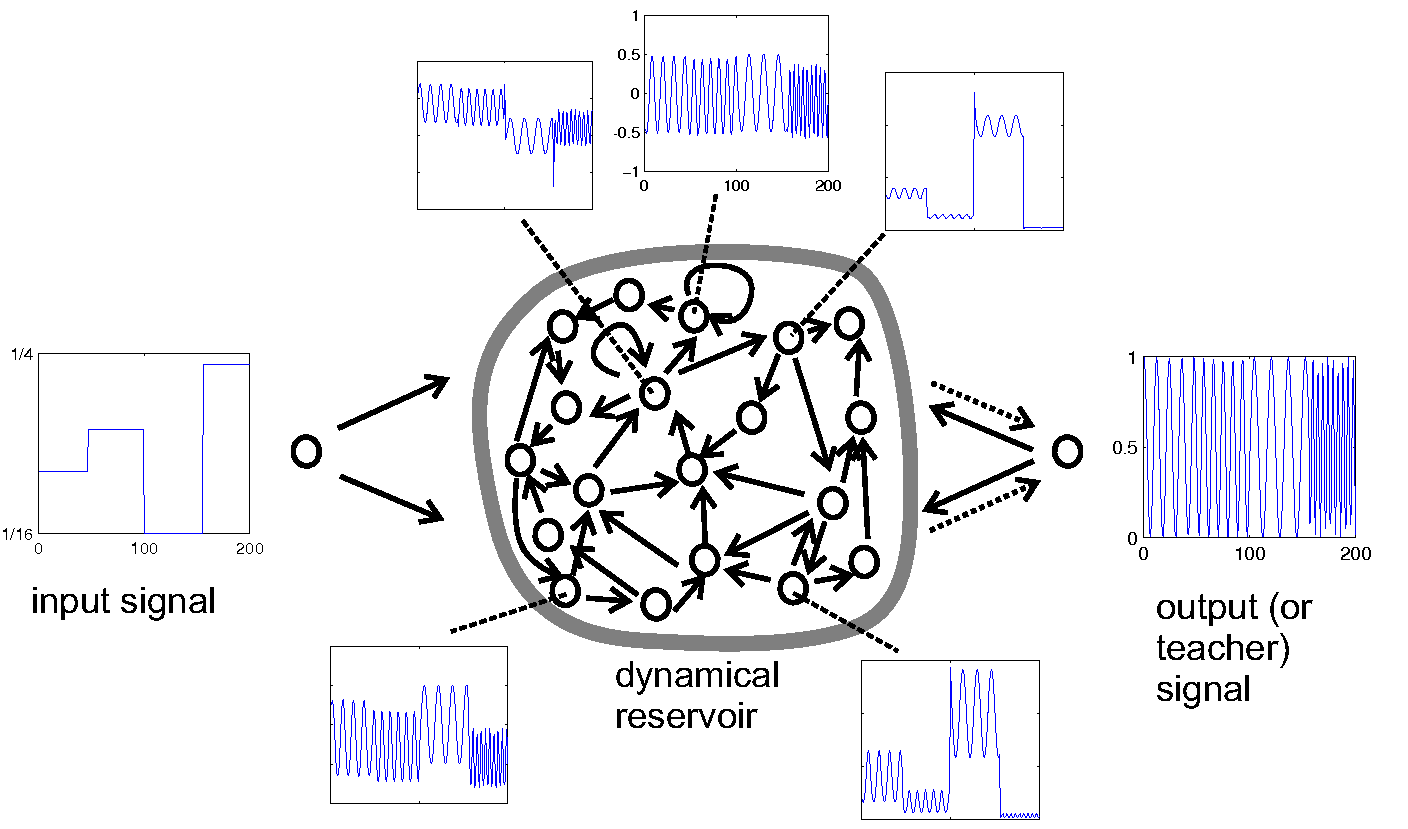
\includegraphics[width=\linewidth]{figures/ESN_diag_FreqGenSchema.png}
                \caption{ESN Diagram.}
            \end{figure}
        \end{column}
        \begin{column}{0.5\textwidth}
            \textbf{Liquid State Machines (LSMs)}
            \begin{itemize}
                \item Spiking neuron models.
                \item Biologically inspired.
                \item Developed by Maass.
            \end{itemize}
            \begin{figure}
                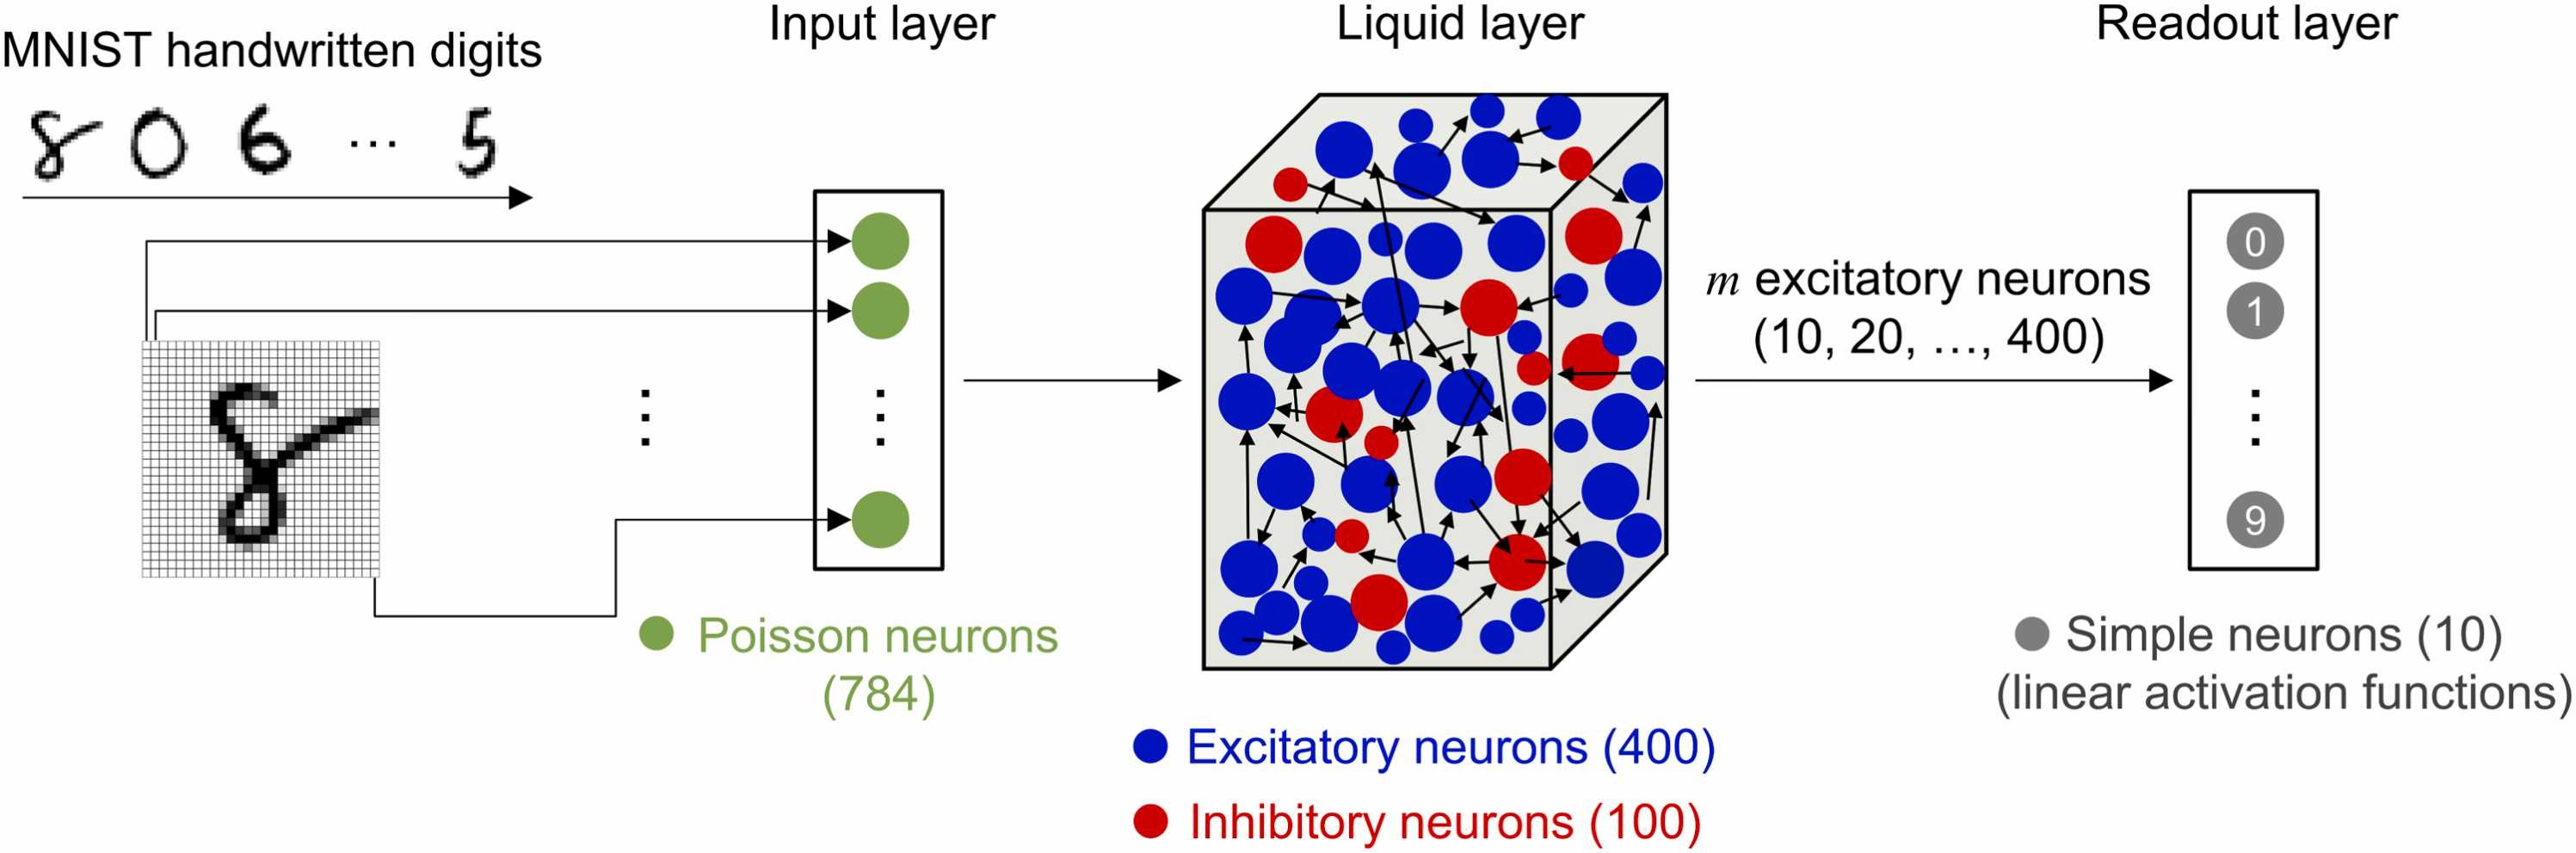
\includegraphics[width=\linewidth]{figures/lsm_diag.png}
                \caption{LSM Diagram.}
            \end{figure}
        \end{column}
    \end{columns}
    \pause\medskip
    \textbf{Physical Reservoir Computing (PRC):} Uses physical systems (optical, mechanical) as reservoirs.
\end{frame}

\begin{frame}
    \frametitle{Training Methodology}
    Simple, efficient process:
    \begin{enumerate}
        \item \textbf{Collect States:} Feed input signals $\mathbf{u}$ into the fixed reservoir and record the resulting states $\mathbf{x}$ over time. Let $G$ be the matrix of collected states.
        \pause
        \item \textbf{Train Readout:} Solve a linear regression problem to find the output weights $\mathbf{W}_{\text{out}}$ that map reservoir states $G$ to the target outputs $Y$.
            \[
            \mathbf{W}_{\text{out}} = Y G^T \left(G G^T + \lambda I\right)^{-1}
            \]
            (Ridge Regression formula, where $\lambda$ is regularization parameter).
        \pause
        \item \textbf{Infer:} Use the trained $\mathbf{W}_{\text{out}}$ to predict outputs for new input sequences based on their corresponding reservoir states.
    \end{enumerate}
\end{frame}

\begin{frame}
    \frametitle{Advantages and Limitations}
    \textbf{Advantages:}
    \begin{itemize}
        \item Very fast training (linear regression).
        \item Avoids gradient issues of RNNs.
        \item Same reservoir potentially usable for multiple tasks (train different readouts).
        \item Enables physical implementations.
    \end{itemize}
    \pause
    \textbf{Limitations:}
    \begin{itemize}
        \item Random initialization offers little control over reservoir function.
        \item Memory capacity limited by reservoir size.
        \item Performance highly dependent on task and hyperparameters.
        \item Sensitivity to choice of reservoir dynamics.
    \end{itemize}
\end{frame}

%%%%%%%%%%%%%%%%%%%%%%%%%%%%%%%%%%%%%%%%%%%%%%%%%%%%%%%%%%%%%%%%%%%%%%
% Section 3: Literature Review
%%%%%%%%%%%%%%%%%%%%%%%%%%%%%%%%%%%%%%%%%%%%%%%%%%%%%%%%%%%%%%%%%%%%%%
\section{Literature Review Highlights}

\begin{frame}
    \frametitle{Key Papers Explored}
    \begin{itemize}
        \item \textbf{RC Introduction [\textit{article\_RC\_intro}]:} Basics of setting up RC, emphasizes training only the output layer.
        \pause
        \item \textbf{RC Limitations [\textit{article\_catch\_22s\_rc}]:} Standard ESNs struggle with complex tasks like basin prediction without long warm-up; Next-Gen RC (NGRC) is better but needs exact system knowledge.
        \pause
        \item \textbf{Discrete Map Reservoirs [\textit{Arun2024}]:} Logistic map with virtual nodes can effectively predict chaotic systems (Lorenz, Rössler) even with noise. Simple maps can work!
        \pause
        \item \textbf{Minimal Physical RC [\textit{Mandal2022}]:} A single driven pendulum's transient dynamics can act as a reservoir for standard tasks. Low-dimensional physical systems have potential.
        \pause
        \item \textbf{Bifurcation Reconstruction [\textit{Itoh2020}]:} Used Extreme Learning Machine (ELM) on noisy time-series from an electronic circuit to reconstruct bifurcation diagrams and Lyapunov exponents robustly.
    \end{itemize}
\end{frame}

%%%%%%%%%%%%%%%%%%%%%%%%%%%%%%%%%%%%%%%%%%%%%%%%%%%%%%%%%%%%%%%%%%%%%%
% Section 4: Implementation and Results
%%%%%%%%%%%%%%%%%%%%%%%%%%%%%%%%%%%%%%%%%%%%%%%%%%%%%%%%%%%%%%%%%%%%%%
\section{Implementation and Results}

\subsection{Pendulum Reservoir}

\begin{frame}
    \frametitle{Experiment 1: Pendulum as Reservoir}
    Inspired by \cite{Mandal2022}.
    \begin{columns}[T]
        \begin{column}{0.5\textwidth}
            \textbf{Setup:}
            \begin{itemize}
                \item Use a simulated driven, damped pendulum.
                \item Input signal = time-varying driving force.
                \item Reservoir state = [angle ($x$), angular velocity ($v$)].
                \item Train linear readout on state history.
            \end{itemize}
            \textbf{Dynamics:}
            \begin{align*}
            \frac{dx}{dt} &= v \\
            \frac{dv}{dt} &= -\frac{g}{l} \sin(x) - k v \\ & \quad + f \, \text{sign}(\sin(\omega t))
            \end{align*}
        \end{column}
        \begin{column}{0.5\textwidth}
            \textbf{Simple Prediction Result:}
            \begin{figure}
                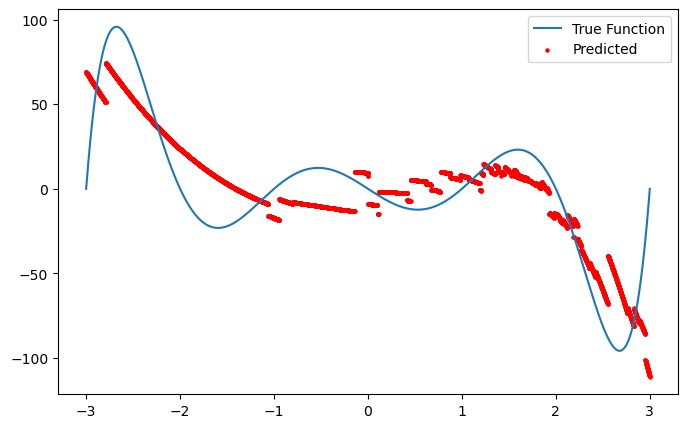
\includegraphics[width=\linewidth]{figures/pendulum_result_0.png}
                \caption{Predicting next state based on previous ($x_{t-1}$). Shows learning capability.}
                \label{fig:pendulum-1-slide}
            \end{figure}
        \end{column}
    \end{columns}
    \textit{Finding: Simple oscillator can work as a reservoir, but results are hyperparameter-sensitive.}
\end{frame}

\begin{frame}
    \frametitle{Pendulum Reservoir: Lorenz System Prediction}
    Task: Predict the Lorenz attractor dynamics using the pendulum reservoir.
    \textbf{Lorenz System:}
    \begin{align*}
        \frac{dx}{dt} &= \sigma (y - x) \\
        \frac{dy}{dt} &= x (\rho - z) - y \\
        \frac{dz}{dt} &= x y - \beta z
    \end{align*}
    ($\sigma=10, \rho=28, \beta=8/3$) \pause
    \textbf{Results:}
    \begin{figure}
        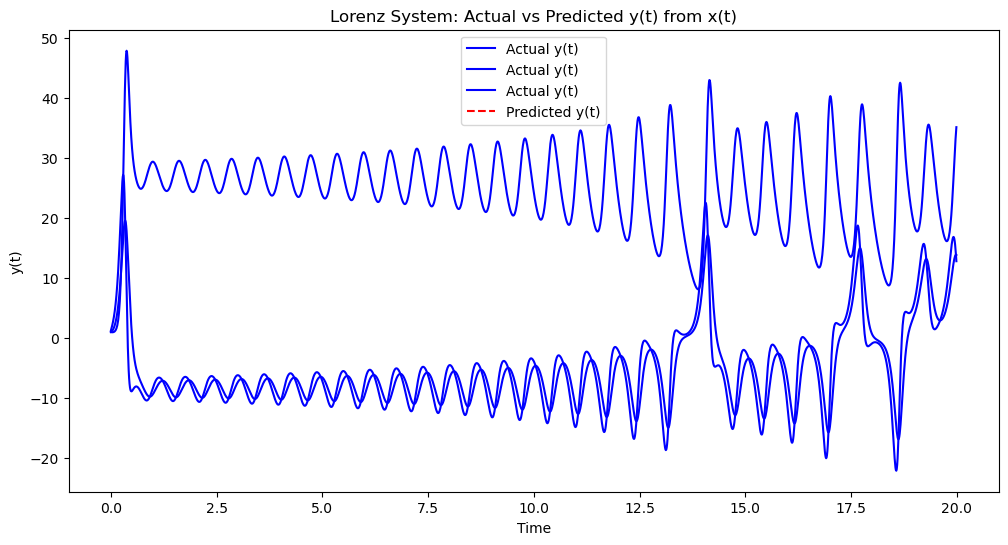
\includegraphics[width=0.9\linewidth]{figures/lorentz_pendulum_1.png}
        \caption{Actual vs Predicted components over time.}
        \label{fig:lorentz_1_slide}
    \end{figure}
\end{frame}

\begin{frame}
    \frametitle{Pendulum Reservoir: Lorenz System Prediction (3D)}
    \begin{figure}
        \centering
        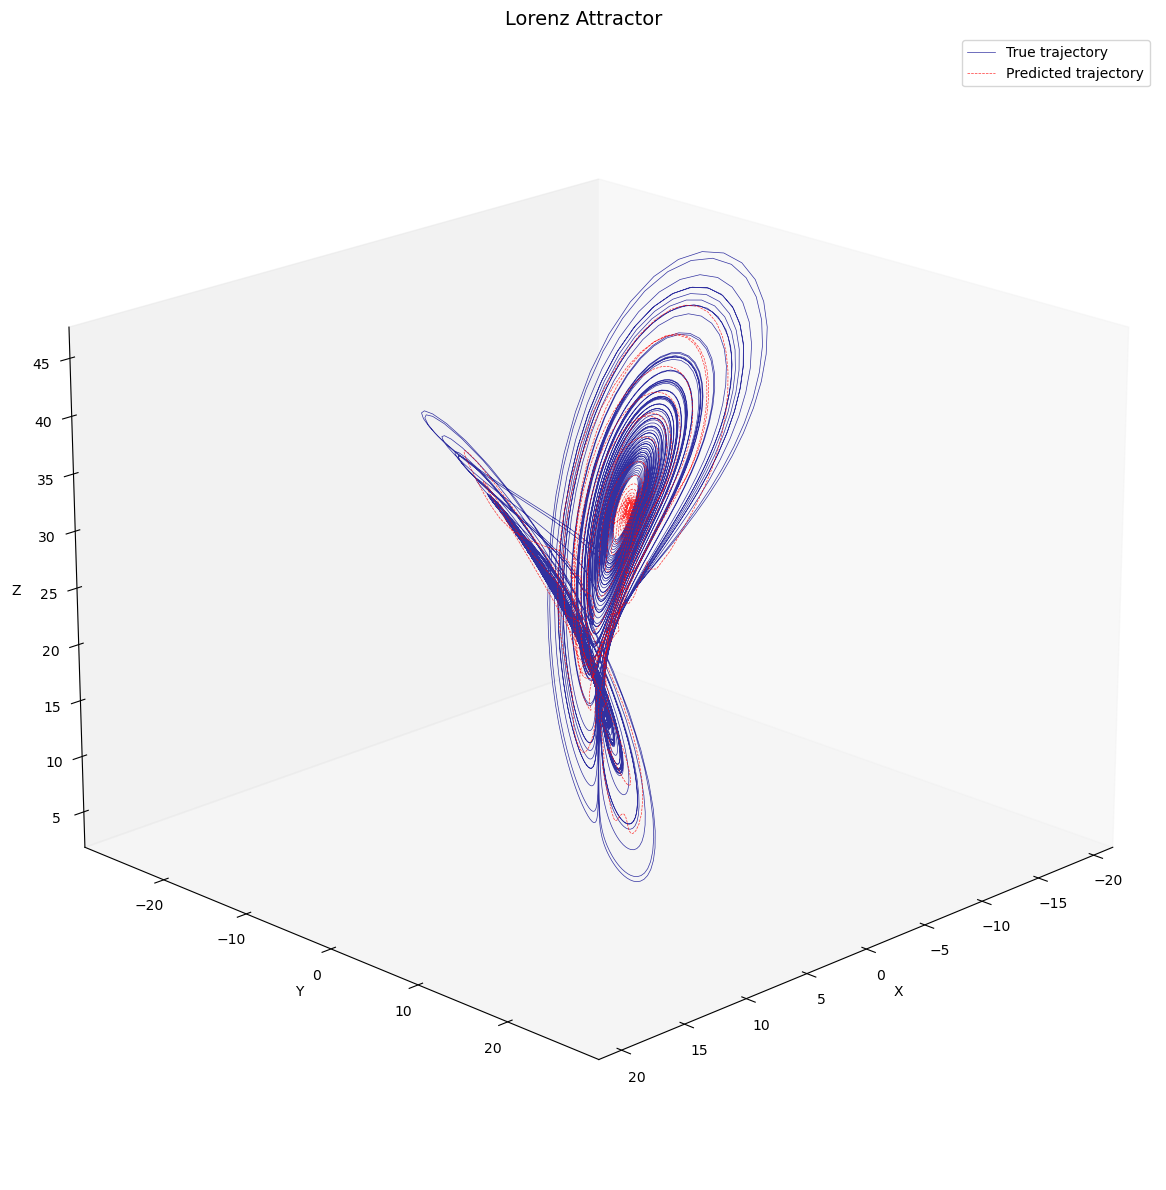
\includegraphics[width=0.8\linewidth]{figures/lorentz_pendulum_2.png}
        \caption{3D plot: True Lorenz attractor (blue) vs Predicted trajectory (orange).}
        \label{fig:lorentz_2_slide}
    \end{figure}
    \textit{Qualitatively captures attractor shape, but deviations exist.}
\end{frame}

\subsection{Logistic Map Reservoir}

\begin{frame}
    \frametitle{Experiment 2: Logistic Map Reservoir}
    Inspired by \cite{Arun2024}.
    \begin{itemize}
        \item Reservoir constructed using iterates of the logistic map: $x_{n+1} = r x_n (1 - x_n)$.
        \item \textbf{Virtual Nodes Technique:} For each input, iterate map multiple times, sample intermediate values to form high-dimensional state vector.
        \item Train linear readout on this state. \pause
        \item \textbf{Benchmark Task (Polynomial):} Predict a 7th-degree polynomial target.
    \end{itemize}
    \begin{figure}
        \centering
        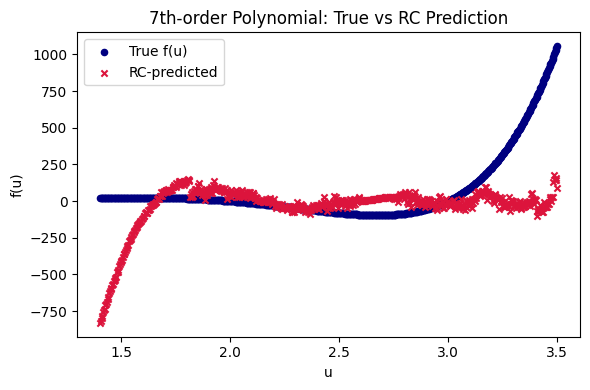
\includegraphics[width=0.7\linewidth]{figures/logistic_7th_degree.png}
        \caption{Logistic map reservoir predicting target polynomial. Shows effectiveness.}
        \label{fig:logistic_map_slide}
    \end{figure}
    \textit{Validates that discrete maps can function as reservoirs.}
\end{frame}

\begin{frame}
    \frametitle{Logistic Map Reservoir: Lorenz System Prediction}
    Same task as before, but using the logistic map reservoir.
    \textbf{Results:}
    \begin{itemize}
        \item Test RMSE (x,y,z): [3.77, 2.94, 8.36]
    \end{itemize}
    \begin{figure}
        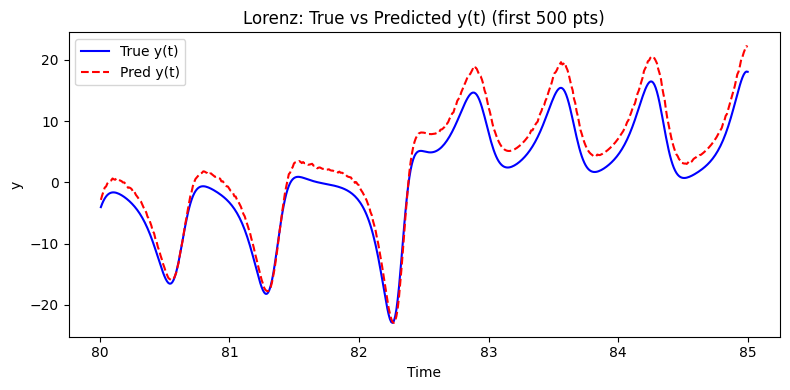
\includegraphics[width=0.9\linewidth]{figures/lorentz_logistic_pred_true.png}
        \caption{Actual vs Predicted components over time.}
        \label{fig:logistic_map_lorenz_slide}
    \end{figure}
\end{frame}

\begin{frame}
    \frametitle{Logistic Map Reservoir: Lorenz System Prediction (Evolution)}
     \begin{figure}
        \centering
        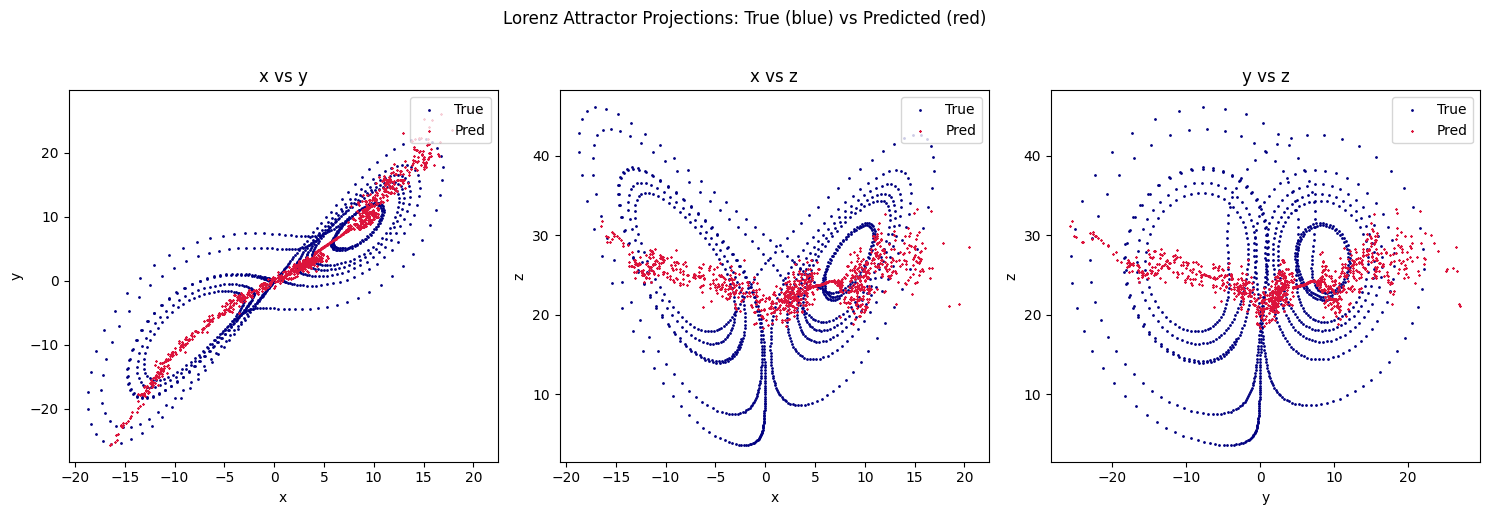
\includegraphics[width=0.9\linewidth]{figures/lorenz_logistic_pred_diagram.png}
        \caption{Evolution of predicted vs true components.}
        \label{fig:logistic_map_lorenz_diag_slide}
    \end{figure}
    \textit{Performance comparable to pendulum reservoir, confirming discrete map viability.}
\end{frame}


\subsection{Bifurcation Reconstruction (ELM + PCA)}

\begin{frame}
    \frametitle{Experiment 3: Bifurcation Reconstruction}
    Inspired by \cite{Itoh2020}, using Logistic Map data.
    \textbf{Goal:} Reconstruct bifurcation diagram from time-series data generated at different parameter values ($\mu$).
    \pause
    \textbf{Procedure:}
    \begin{enumerate}
        \item Generate noisy time-series data for logistic map across a range of $\mu$.
        \item For each $\mu$, train an ELM (like RC, fixed random hidden layer) to predict $x_{t+1}$ from $x_t$. Collect output weights $\mathbf{W}^{\mathrm{out}}_{\mu}$.
        \item Apply PCA to the collected $\mathbf{W}^{\mathrm{out}}_{\mu}$ matrices to estimate the underlying parameter space.
        \item Use the trained ELMs (or a regressor trained on PCA features + $\mu$) to generate attractor points across the estimated parameter range.
    \end{enumerate}
\end{frame}

\begin{frame}
    \frametitle{Initial Reconstruction Attempt (ELM + PCA)}
    \begin{figure}
        \centering
        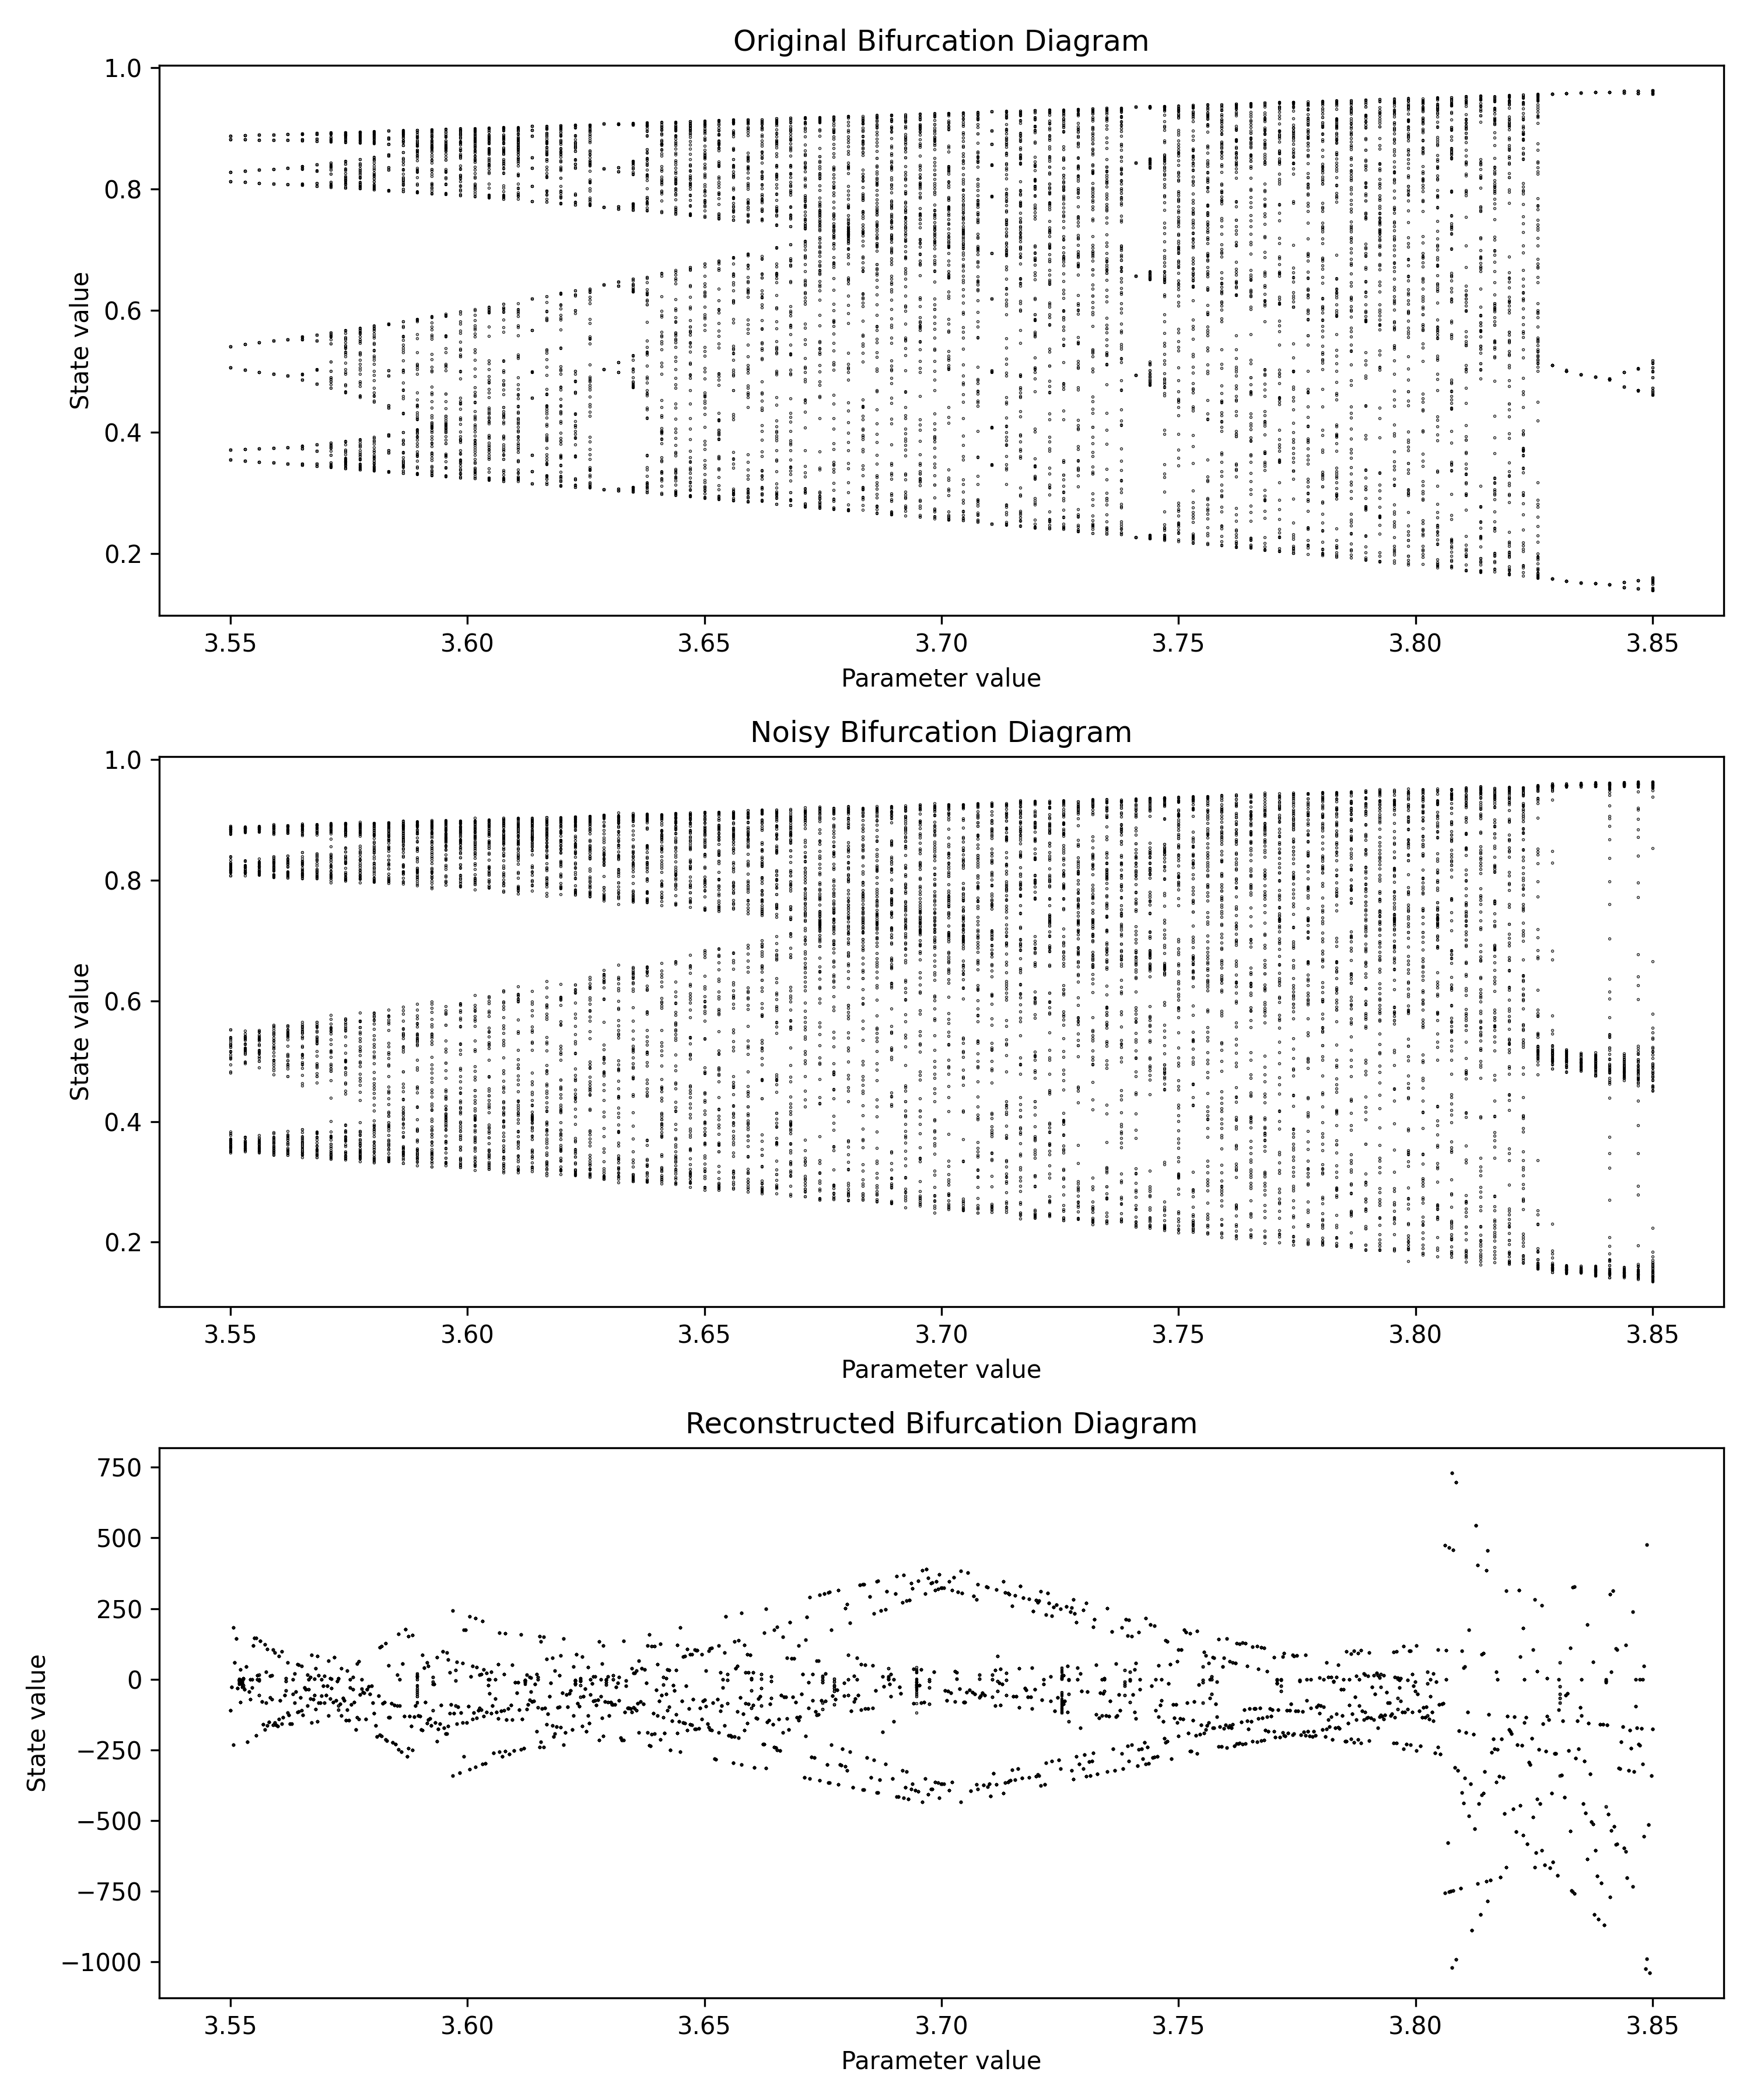
\includegraphics[width=0.9\linewidth]{figures/bd_reconstruction_elm.png}
        \caption{First attempt at reconstruction. Incomplete, noisy, missing branches.}
        \label{fig:bifurcation_slide}
    \end{figure}
    \textit{Initial results were poor. Challenges: sensitivity, noise, potentially incorrect implementation details vs paper.}
\end{frame}

\begin{frame}
    \frametitle{Improved Reconstruction Results (ELM + PCA)}
    After fine-tuning and fixing implementation issues:
     \begin{figure}
        \centering
        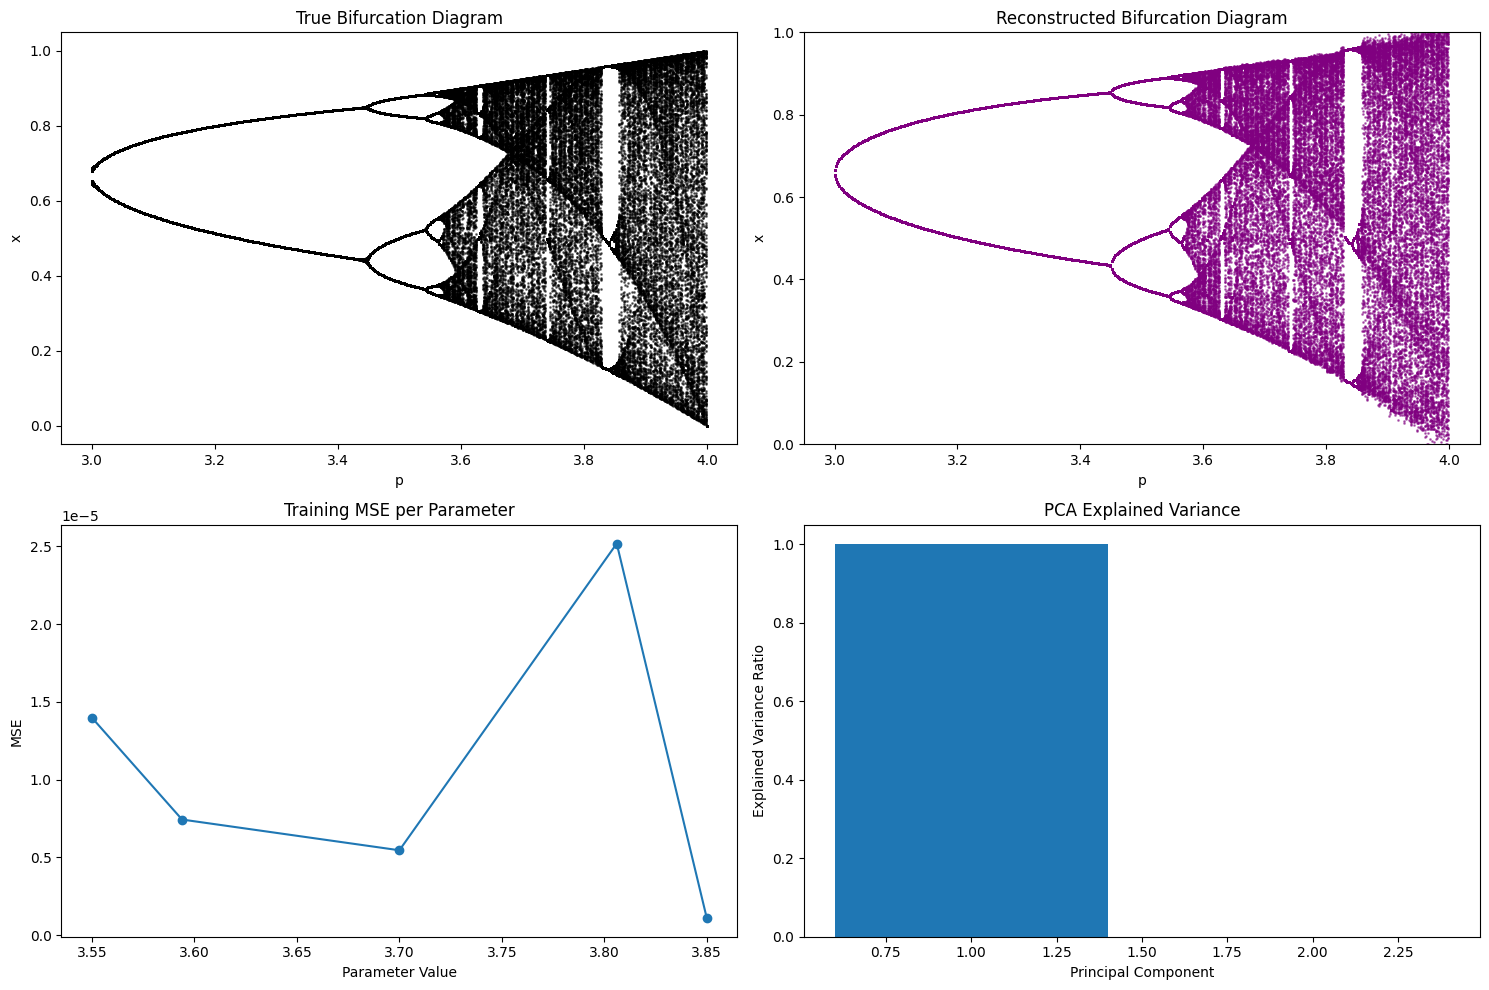
\includegraphics[width=0.8\linewidth]{figures/bd_1_results.png}
        \caption{Improved reconstruction. Training MSE: 1.06e-05.}
        \label{fig:bd_1_slide}
    \end{figure}
    \textit{Much better, capturing the main period-doubling structure.}
\end{frame}

\begin{frame}
    \frametitle{Reconstruction Results (ELM + PCA): Return Plot & Overlap}
    \begin{columns}[T]
        \begin{column}{0.5\textwidth}
            \textbf{Return Plot ($x_{t+1}$ vs $x_t$):}
            \begin{figure}
                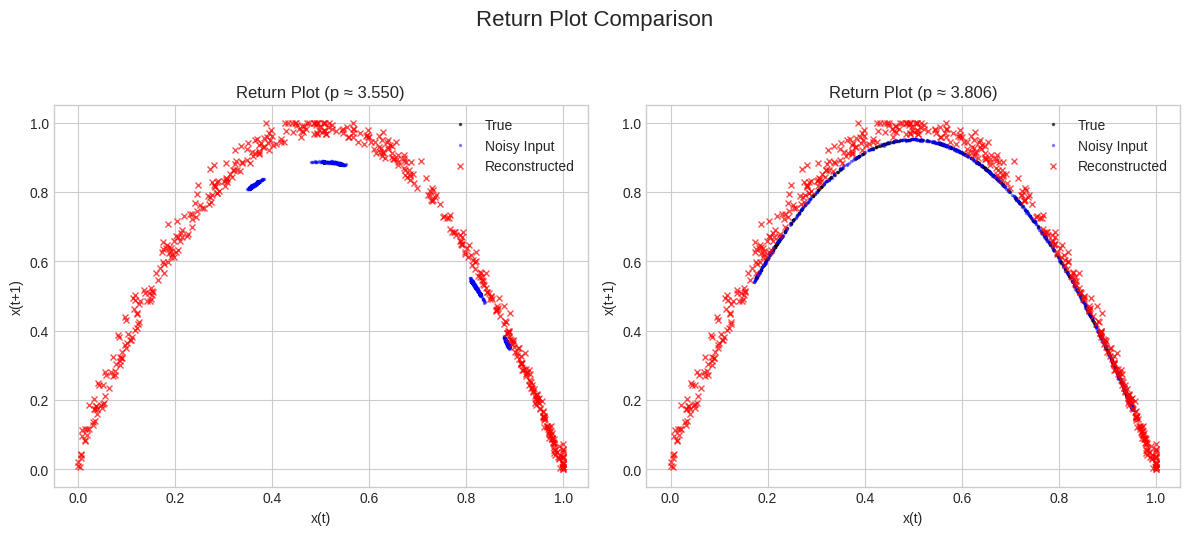
\includegraphics[width=\linewidth]{figures/bd_return_plot_2.png}
                \caption{Reconstructed return plot matches true structure well.}
                 \label{fig:bd_2_slide}
            \end{figure}
        \end{column}
        \begin{column}{0.5\textwidth}
            \textbf{Overlapped Bifurcation Diagrams:}
             \begin{figure}
                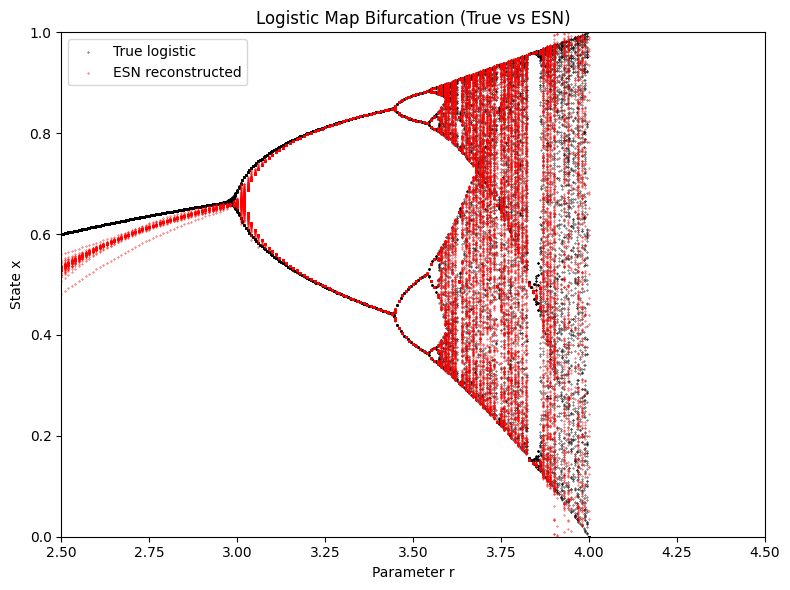
\includegraphics[width=\linewidth]{figures/bf_3_results_overlapped.png}
                \caption{True (blue) vs Predicted (orange). Good match in trained region, poor extrapolation.}
                 \label{fig:bd_3_slide}
            \end{figure}
        \end{column}
    \end{columns}
\end{frame}

\begin{frame}
    \frametitle{Reconstruction Results (ELM + PCA): Lyapunov & PCA Analysis}
    \begin{columns}[T]
        \begin{column}{0.5\textwidth}
            \textbf{Approximate Lyapunov Exponents:}
            \begin{figure}
                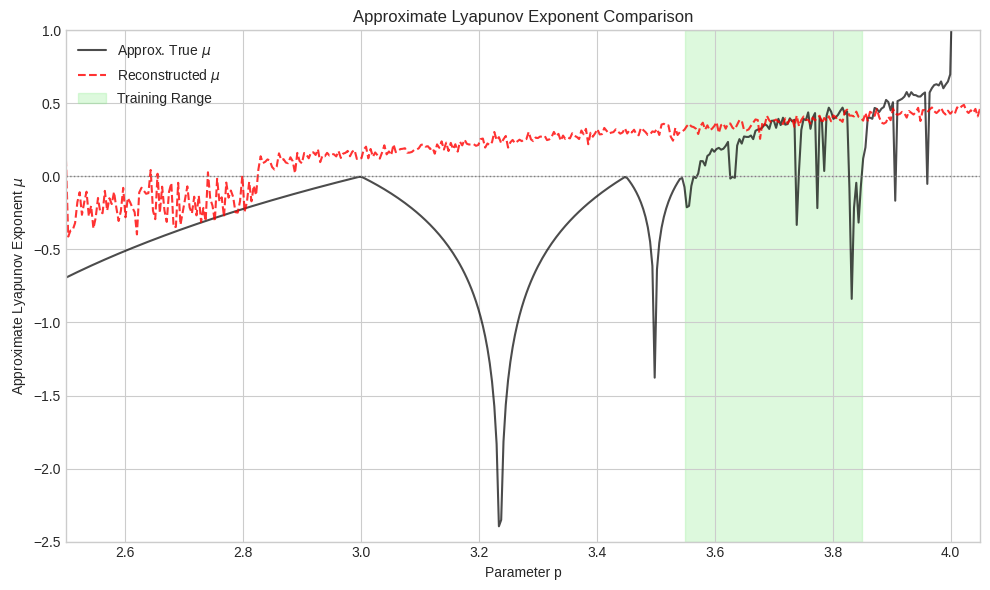
\includegraphics[width=\linewidth]{figures/lyapanov_bd_rd.png}
                \caption{Estimating dynamics (positive = chaos) vs parameter. Green = training range.}
                 \label{fig:lypanov_bd_rc_slide}
            \end{figure}
        \end{column}
        \begin{column}{0.5\textwidth}
            \textbf{PCA Component Analysis:}
             \begin{figure}
                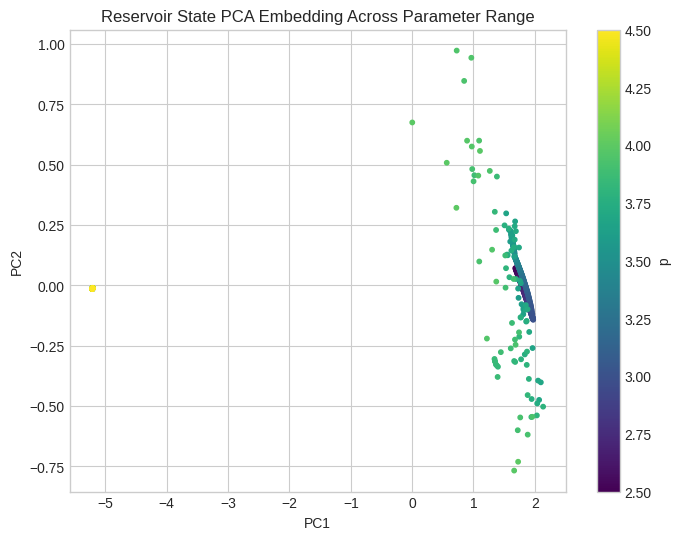
\includegraphics[width=\linewidth]{figures/bd_elm_pca_analysis.png}
                \caption{PCA components vs parameter show correlation, potentially identifying parameter space.}
                 \label{fig:bd_4_slide}
            \end{figure}
        \end{column}
    \end{columns}
\end{frame}


\subsection{Bifurcation Reconstruction (LSTM)}

\begin{frame}
    \frametitle{Alternative: LSTM for Reconstruction}
    \textbf{Problem:} Initial RC/ELM approaches struggled to cleanly reconstruct bifurcation diagrams directly or extrapolate well. A single fixed reservoir might average dynamics across parameters.
    \pause
    \textbf{Alternative Approach:} Use a Long Short-Term Memory (LSTM) network.
    \begin{columns}[T]
         \begin{column}{0.4\textwidth}
            \textbf{Key Differences:}
            \begin{itemize}
                \item LSTM is fully trainable (incl. recurrent weights).
                \item Parameter $p$ is given as \textit{explicit input} along with state $x_t$.
                \item Learns conditional dynamics: $\hat{x}_{t+1} = g_{\text{LSTM}}(x_t, p; \theta)$.
                \item Trained on data from *all* parameters simultaneously.
            \end{itemize}
         \end{column}
         \begin{column}{0.6\textwidth}
              \begin{figure}
                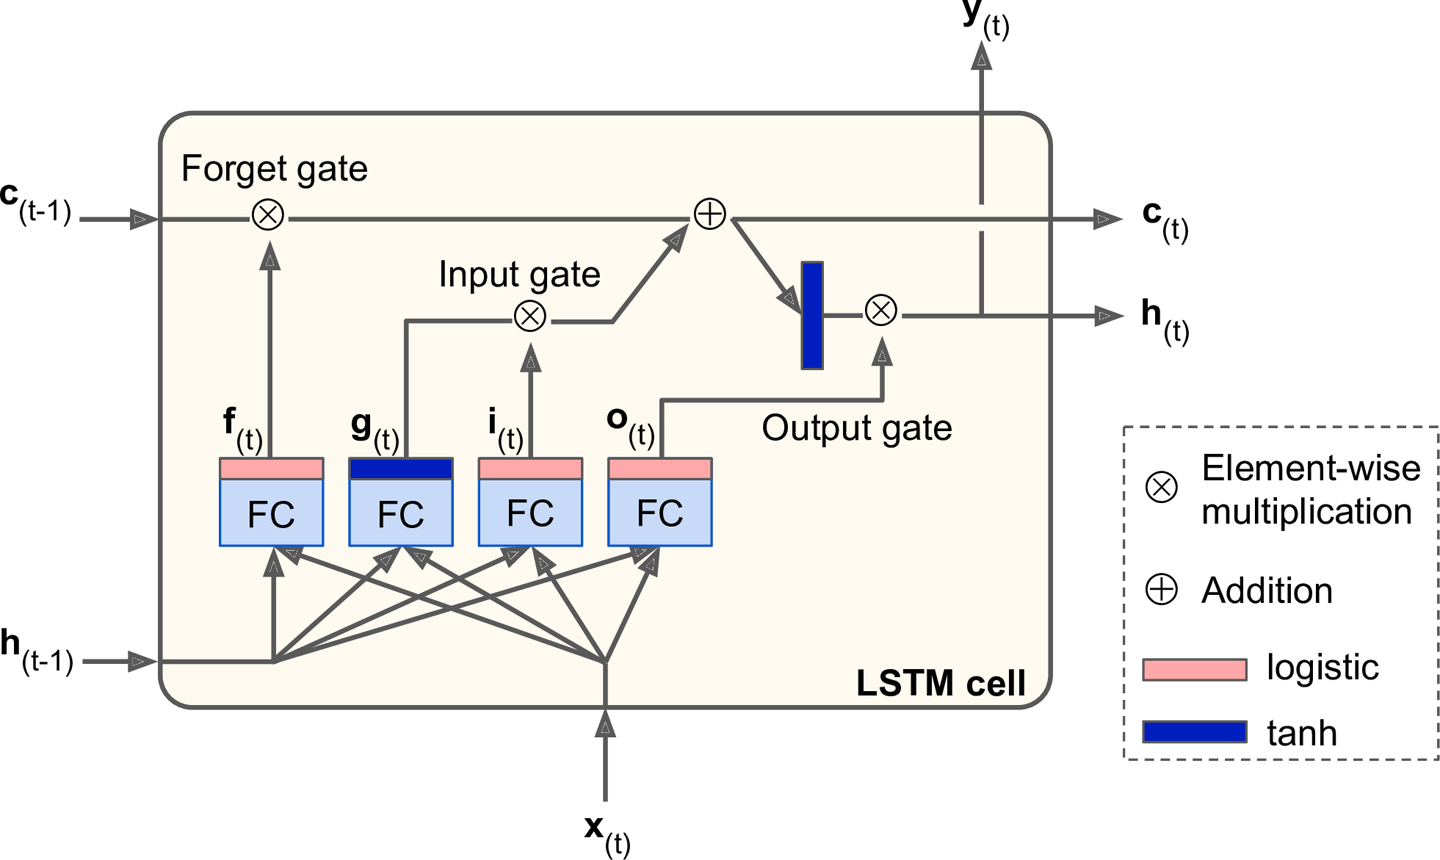
\includegraphics[width=0.8\linewidth]{figures/LSTM_arch.png}
                \caption{LSTM Cell Architecture.}
                 \label{fig:lstm_arch_slide}
            \end{figure}
         \end{column}
    \end{columns}
\end{frame}

\begin{frame}
    \frametitle{LSTM Reconstruction Results: Bifurcation Diagram}
    \begin{figure}
        \centering
        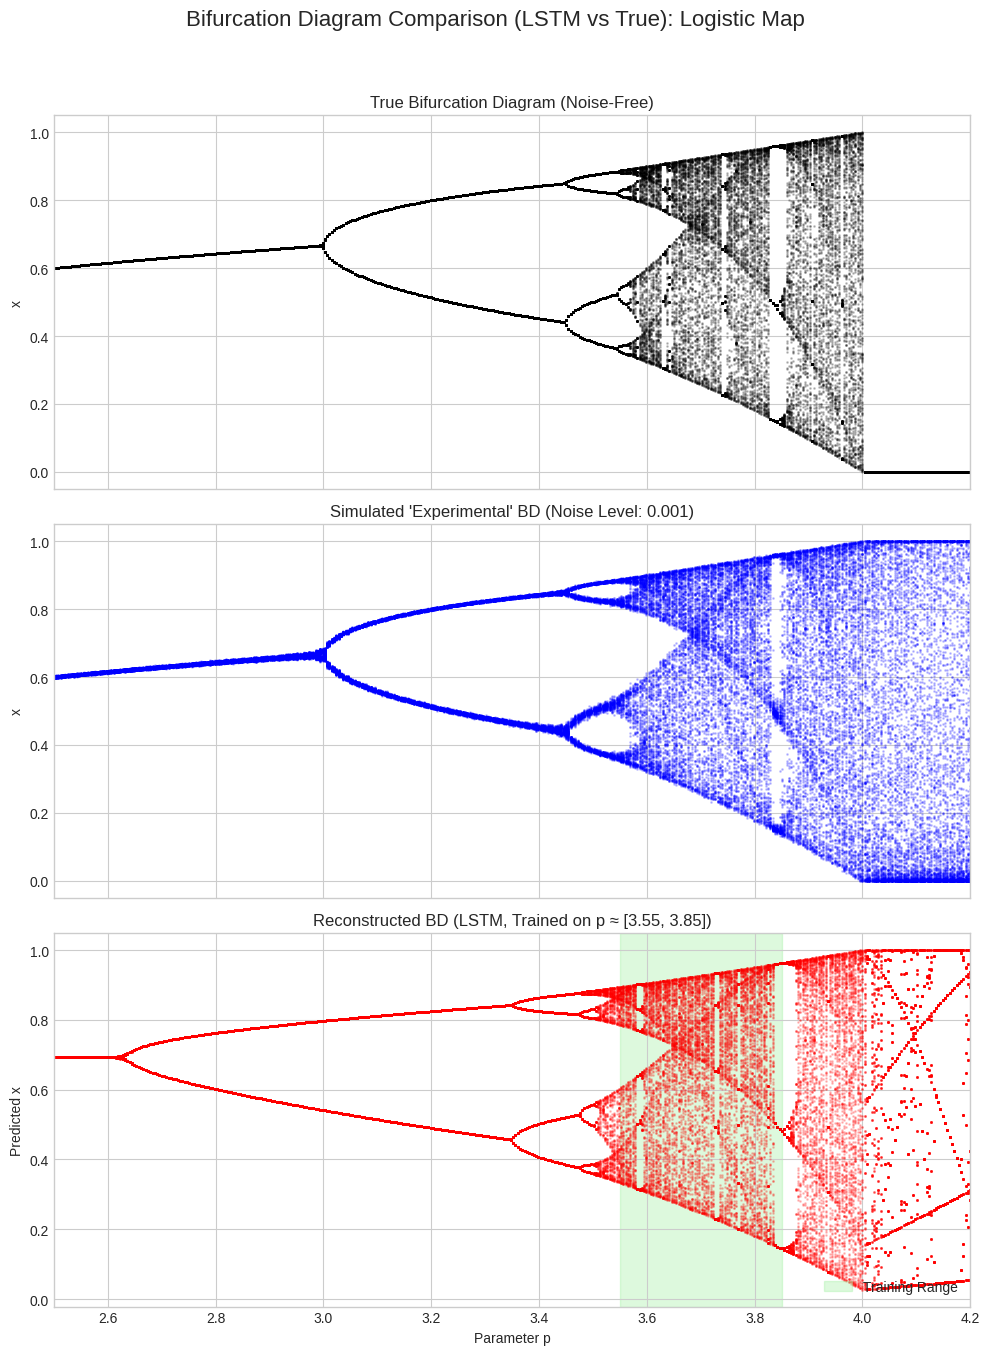
\includegraphics[width=1.0\linewidth]{figures/lstm_bd_1.png}
        \caption{LSTM reconstruction (orange) vs True (blue). Green = training parameter range. Good extrapolation!}
        \label{fig:lstm_bd_1_slide}
    \end{figure}
    \textit{LSTM successfully learns parameter-dependent dynamics and extrapolates reasonably well.}
\end{frame}

\begin{frame}
    \frametitle{LSTM Reconstruction Results: Return Plot & Lyapunov}
     \begin{columns}[T]
        \begin{column}{0.5\textwidth}
            \textbf{Return Plot ($x_{t+1}$ vs $x_t$):}
             \begin{figure}
                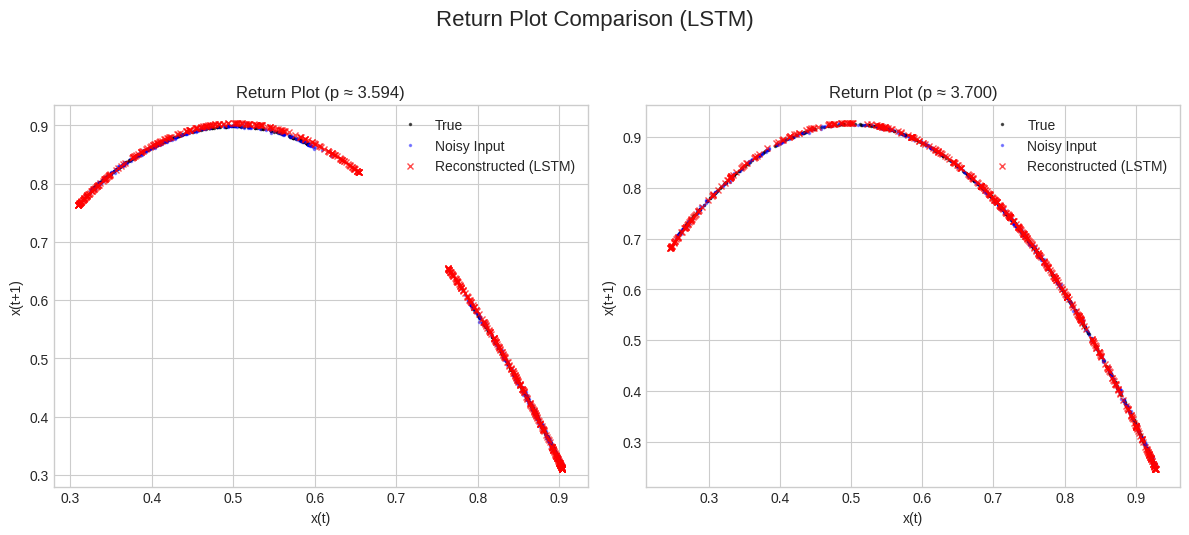
\includegraphics[width=\linewidth]{figures/lstm_bd_2.png}
                \caption{Reconstructed return plots across parameters.}
                 \label{fig:lstm_bd_2_slide}
            \end{figure}
        \end{column}
        \begin{column}{0.5\textwidth}
            \textbf{Approximate Lyapunov Exponents:}
             \begin{figure}
                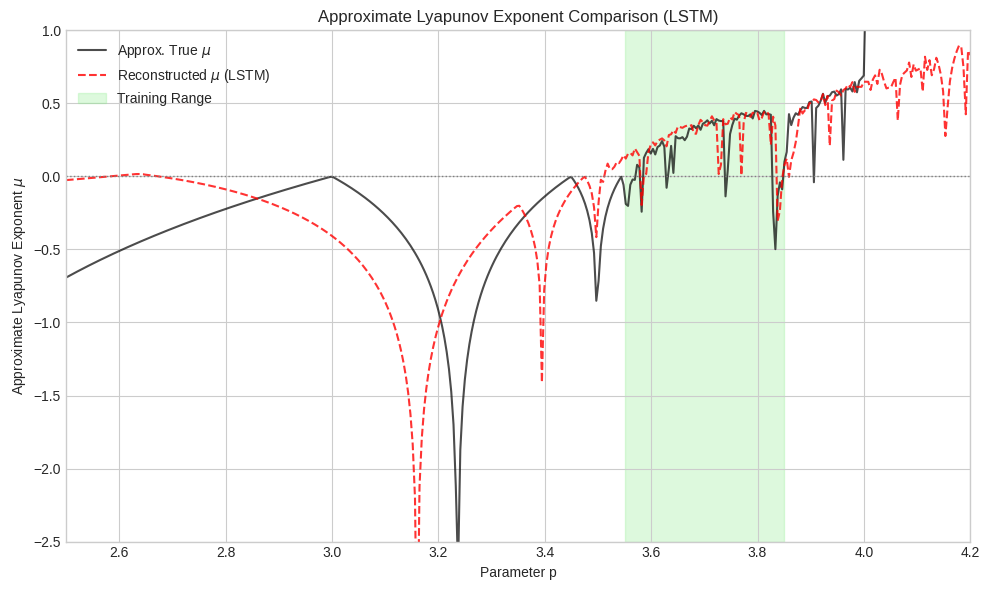
\includegraphics[width=\linewidth]{figures/lstm_bd_3.png}
                \caption{Estimated exponents match trends well, including extrapolation.}
                 \label{fig:lstm_bd_3_lyap_slide}
            \end{figure}
        \end{column}
    \end{columns}
\end{frame}

\begin{frame}
    \frametitle{RC/ELM vs LSTM: Training Time Trade-off}
    \textbf{Performance Comparison for Bifurcation Reconstruction:}
    \begin{itemize}
        \item \textbf{ELM (RC-like):}
            \begin{itemize}
                \item Training Time: \textbf{< 1 second} (Linear regression is fast!)
                \item Reconstruction Quality: Good within training range, poor extrapolation, sensitive setup (PCA step).
            \end{itemize}
        \pause
        \item \textbf{LSTM (RNN):}
            \begin{itemize}
                \item Training Time: \textbf{~46 seconds} (Backpropagation is slower)
                \item Reconstruction Quality: Very good, including extrapolation, simpler setup (parameter as input).
            \end{itemize}
    \end{itemize}
    \pause
    \textbf{Takeaway:} RC offers huge speed-up but might lack flexibility for complex conditional tasks compared to fully trained RNNs, especially when compute is available. Newer sequence models (Transformers, Mamba) offer other alternatives.
\end{frame}

%%%%%%%%%%%%%%%%%%%%%%%%%%%%%%%%%%%%%%%%%%%%%%%%%%%%%%%%%%%%%%%%%%%%%%
% Section 5: Conclusion
%%%%%%%%%%%%%%%%%%%%%%%%%%%%%%%%%%%%%%%%%%%%%%%%%%%%%%%%%%%%%%%%%%%%%%
\section{Conclusion}

\begin{frame}
    \frametitle{Conclusion}
    \begin{itemize}
        \item Explored Reservoir Computing (RC) for analyzing noisy time-series, focusing on bifurcation diagram reconstruction using ELM+PCA.
        \pause
        \item RC/ELM could capture broad dynamics (period doubling) but struggled with fine chaotic structures and extrapolation.
            \begin{itemize}
                \item Highlights challenges with noise, hyperparameter sensitivity.
            \end{itemize}
        \pause
        \item Gained practical insights into RC principles:
            \begin{itemize}
                \item Massive training efficiency vs RNNs.
                \item Potential for modeling physical systems.
            \end{itemize}
        \pause
        \item Fully trainable RNNs (like LSTM), explicitly using the parameter as input, showed superior performance for this specific reconstruction task, despite longer training time.
        \pause
        \item Suggests that for complex conditional modeling where compute is less constrained, traditional RNNs (or newer architectures) might be more suitable than standard RC.
    \end{itemize}
\end{frame}

%%%%%%%%%%%%%%%%%%%%%%%%%%%%%%%%%%%%%%%%%%%%%%%%%%%%%%%%%%%%%%%%%%%%%%
% Section 6: Future Work
%%%%%%%%%%%%%%%%%%%%%%%%%%%%%%%%%%%%%%%%%%%%%%%%%%%%%%%%%%%%%%%%%%%%%%
\section{Future Work}

\begin{frame}
    \frametitle{Future Work}
    \begin{itemize}
        \item \textbf{Optimize RC/ELM:} Thorough hyperparameter tuning (size, spectral radius, regularization) potentially using Bayesian Optimization.
        \pause
        \item \textbf{Broader Systems:} Apply to higher-dimensional maps, continuous systems (ODEs), different bifurcation types (Hopf, saddle-node), coupled systems.
        \pause
        \item \textbf{Alternative Architectures:} Explore deep reservoirs, different readout mechanisms.
        \pause
        \item \textbf{Physical Validation:} Test reconstruction techniques on real experimental data (electronic circuits, pendulums) - the original motivation.
    \end{itemize}
\end{frame}

%%%%%%%%%%%%%%%%%%%%%%%%%%%%%%%%%%%%%%%%%%%%%%%%%%%%%%%%%%%%%%%%%%%%%%
% Acknowledgements & References
%%%%%%%%%%%%%%%%%%%%%%%%%%%%%%%%%%%%%%%%%%%%%%%%%%%%%%%%%%%%%%%%%%%%%%
\section*{Acknowledgements \& Code}

\begin{frame}
    \frametitle{Acknowledgement}
    \Large
    Thank you to \textbf{Prof. Gaurav Dar} for guidance, insights, and motivation throughout this project.
\end{frame}

\begin{frame}
    \frametitle{Code Availability}
    \Large
    The complete code with experiments is available on GitHub:

    \bigskip
    \url{https://github.com/vimarsh244/ResorvoirComputing_SOP}

    \bigskip
    \textit{(Full references are available in the project report)}
\end{frame}


\end{document}
